%! TEX root = ../main.tex

\section{PE формат}
Исполняемые файлы в системе Windows имеет общую сигнатуру, называемую
PE (Portable Executable). В PE формате содержится различная информация о
исполняемом файле, как например: таблицы импорта и экспорта, информация о
различных секциях, точка входа и так далее. Структура PE формата представлена на
рисунке \ref{fig:PE}.
\begin{figure}[htb]
  \centering
  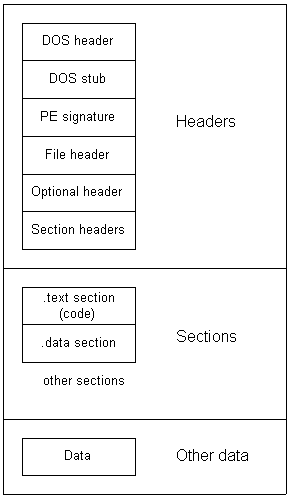
\includegraphics[width=0.45\textwidth]{PE.png}
  \caption{Формат PE}
  \label{fig:PE}
\end{figure}

Рассмотрим те части PE формата, которые будут использованы в данной работе.
Первым идет MS-DOS заголовок, первыми двумя байтами которой является сигнатура
"MZ". Большая часть полей данного заголовка предназначены для запуска из-под
DOS. Для дальнейшей работы, кроме проверки сигнатуры, потребуется поле
\verb!e_lfanew!, в котором содержится указатель на начало PE-заголовка.

PE-заголовок также имеет свою сигнатуру, которую необходимо проверить на
корректность, а именно четыре байта "PE\textbackslash0\textbackslash0". В данном
разделе хранится количество секций \verb!NumberOfSection!, а также размер
идущего за следующим опционального заголовка в байтах
\verb!SizeOfOptionalHeader!.

Далее расположен опциональный заголовок. Данный раздел содержит смещение адреса
входа относительно базового адреса загрузки файла --- \\
\verb!AddresOfEntryPoint!, рекомендуемый базовый адрес загрузки файла
\verb!ImageBase!, количество элементов в таблице \verb!DATA_DIRECTORY! ---
\verb!NumberOfRvaAndSizes!.  \verb!DATA_DIRECTORY! представляет собой таблицу,
каждый элемент которой представляет из себя структуру из двух полей, а именно
виртуального адреса тех данных, на который указывает данный элемент, и их размер. 

Далее идет таблица секций. Для каждой секции в этой таблице приведена следующая
информация:
\begin{itemize}
  \item \verb!Name! --- имя секции. 
  \item \verb!VirtualAddress! --- виртуальный адрес секции в памяти.
  \item \verb!PointerToRawData! --- указатель на данные в файле.
  \item \verb!VirtualSize! --- размер, занимаемый секцией в памяти.
  \item \verb!Characteristics! --- свойства секции. Так, например, секция,
    которую можно запустить на выполнение должна обладать свойством
    \\ \verb!IMAGE_SCN_CNT_CODE!.
\end{itemize}

В данной работе также будет использована секция \verb!.reloc!, в которой
содержится таблица базовых смещений. В целях безопасности исполняемый файл может
быть загружен по случайному адресу. Соответственно, адреса, используемые в коде
программы, необходимо изменить в соответствии с базовым адресом загрузки.
Информация о всех местах, которые необходимо скорректировать, содержится с
таблице базовых смещений. Таблица состоит из блоков. Первые четыре байта каждого
блока содержат виртуальный адрес, относительно которого заданы записи смещений.
Следующие четыре байта содержат размер блока в байтах. Оставшееся место в блоке
занимают записи смещений. Каждая запись занимает два байта, первые четыре бита
которой --- тип смещения, а оставшиеся двенадцать бит задают смещение
относительно адреса, указанного в первых четырех байтах блока.
